% !TeX program = pdflatex
% NOMS 2027 working manuscript v8 (readability and scientific narrative revision of Sections V--VII). IEEE conference format (official template, 2024-06-28).
% Compile this file directly using pdfLaTeX.
\documentclass[conference]{IEEEtran}
% \IEEEoverridecommandlockouts % Enable only if a funding footnote requires it.
\usepackage{cite}
\usepackage{amsmath,amssymb,amsfonts}
\usepackage{algorithmic}
\usepackage{graphicx}
\usepackage{tikz}
\usetikzlibrary{arrows.meta,calc,shapes.geometric}
\usepackage{textcomp}
\usepackage{xcolor}
\def\BibTeX{{\rm B\kern-.05em{\sc i\kern-.025em b}\kern-.08em
    T\kern-.1667em\lower.7ex\hbox{E}\kern-.125emX}}

% Manuscript-specific semantic macros (do not change IEEE page geometry or fonts).
\newcommand{\QUERY}{\textsc{Query}}
\newcommand{\REFRESH}{\textsc{Refresh}}
\newcommand{\SKIP}{\textsc{Skip}}
\newcommand{\STOP}{\textsc{Stop}}

\title{Intent-Aware Sequential Resource Discovery\\under Uncertain Domain Knowledge}

\author{\IEEEauthorblockN{D\'aniel Ficzere\IEEEauthorrefmark{1}\IEEEauthorrefmark{2},
Attila Frank\'o\IEEEauthorrefmark{1},
Gergely Holl\'osi\IEEEauthorrefmark{1},
P\'al Varga\IEEEauthorrefmark{1},
J\'ozsef B\'ir\'o\IEEEauthorrefmark{1}}
\IEEEauthorblockA{\IEEEauthorrefmark{1}Department of Telecommunications and Artificial Intelligence,\\
Budapest University of Technology and Economics, Budapest, Hungary}
\IEEEauthorblockA{\IEEEauthorrefmark{2}AI \& IIoT Division, AITIA International Inc., Budapest, Hungary}
}
\begin{document}
\maketitle

\begin{abstract}
Federated network and edge managers often know which domains may host resources satisfying an intent, but not whether such resources are currently available. We model discovery as a sequential decision about information acquisition: a costly domain query establishes feasibility, while a cheaper, imperfect refresh changes the estimated likelihood of finding a suitable resource. Search may terminate without success only when the model assigns at most a specified probability $\varepsilon$ to the existence of a suitable resource in the domains not ruled out. We derive conditions for efficient query ordering, screening, and refresh-induced reordering, and develop PSA1-S, a skip-aware rollout with exact small-problem continuation and selective lookahead. On 60 independently generated synthetic problems with 10--12 domains, PSA1-S has a 3.17\% mean expected-cost gap to exact optimization and saves 18.02\% on average against the optimal policy without refresh. Replays of Microsoft Philly and Alibaba-2018 resource telemetry also show savings when the model permits no risk of overlooking a suitable domain. With nonzero risk allowances, however, observed misses can exceed the model-based bound. This highlights the importance of belief calibration before operational deployment.
\end{abstract}

\begin{IEEEkeywords}
intent-based networking, resource discovery, network management,
sequential decision making, value of information, edge computing
\end{IEEEkeywords}

\section{Introduction}
\label{sec:intro}
Intent-based management allows operators to specify service requirements rather than a sequence of low-level configuration commands~\cite{leivadeas2023survey,etsi2024zsm}. An intent may, for example, require compute capacity, sufficient memory and a latency limit. In a federated edge or network-management system, resources satisfying these requirements may be spread across several independently managed domains. A controller often knows which domains advertise potentially relevant resource classes, but their detailed resource status may be incomplete or outdated. It must decide where to look before it can choose a service placement or initiate orchestration.

Looking for a resource has a cost. A detailed domain \QUERY{} can determine whether the domain currently contains a suitable resource, but it incurs signalling, processing or administrative overhead. A cheaper \REFRESH{} of a domain summary offers less precise information. It can nevertheless be useful: an unfavorable observation may justify leaving a domain unexamined, while a favorable one may make that domain the best candidate to query next. Crucially, a refresh can save work even when the controller is not allowed to overlook any suitable resource. It may change the order of queries, allowing the search to succeed earlier on average.

The controller must therefore make a sequence of linked decisions. Querying every domain can waste effort after an early success. Refreshing all summaries in advance can waste effort for the same reason. Conversely, abandoning a domain just because it appears unlikely to contain a suitable resource may miss an opportunity. We make this trade-off explicit: an unsuccessful search may stop only when the estimated probability that \emph{at least one domain not ruled out by an exact query contains a suitable resource} is sufficiently small. This probability is updated as observations arrive. It depends on the assumed belief model, so a nominal stopping bound is not by itself a guarantee of the observed miss frequency.

We study one fixed intent requiring one suitable resource. The controller starts with domain-level feasibility probabilities and chooses between exact queries, imperfect refreshes, and eventual termination. Our goal is to minimize the expected cost of information acquisition while bounding, at each unsuccessful termination, the model-posterior probability of overlooking a feasible domain by $\varepsilon$. This combines several established ideas from resource discovery, freshness-aware information acquisition and sequential testing~\cite{murturi2022metadata,chiariotti2022qaoi,gkenosis2022sbfe,wei2017imperfect}. The question is how to combine them into a tractable, risk-aware decision policy for federated resource discovery.

The main contributions are as follows:
\begin{itemize}
\item \textbf{A unified decision model.} We formulate the joint choice of exact \QUERY{}, imperfect \REFRESH{} and risk-constrained \STOP{}. We give an exact dynamic-programming benchmark and show why permanently skipping a domain need not be represented as a separate action in that benchmark.
\item \textbf{Structural results and a scalable policy.} We establish the scope of query-ordering and screening rules, and show how a refresh can be valuable solely by changing query order. These insights support PSA1-S, which combines inexpensive skip-aware planning, exact continuation on small remaining problems, and selective deeper evaluation of competing actions.
\item \textbf{Complementary empirical evidence.} Controlled synthetic experiments measure approximation quality and decision time. Chronological replays of Microsoft Philly GPU and Alibaba-2018 CPU--memory measurements test whether information refinement can save discovery cost when feasibility is derived from real telemetry. Observed misses are reported separately from the probabilities predicted by the model.
\end{itemize}

These evaluations test different aspects of the method. Synthetic problems with 10--12 domains are large enough to exercise the selective lookahead mechanism, so they inform its accuracy--computation trade-off. The telemetry replays contain four domains and are therefore solved by the exact small-problem component of PSA1-S. They provide evidence about the value of imperfect information, but not about selective lookahead in operational systems. Section~\ref{sec:related} reviews the foundations. Sections~\ref{sec:model}--\ref{sec:algorithms} present the model, structural results and algorithm. Section~\ref{sec:eval} evaluates them, while Section~\ref{sec:discussion} discusses their scope. Proofs and additional implementation and reproduction details appear in the appendices.

\section{Related Work}
\label{sec:related}
\paragraph{Intent-driven management and federated discovery}
Intent-based networking treats the interpretation, translation, deployment and assurance of intents as related management functions~\cite{leivadeas2023survey}. Knowledge-driven intent life-cycle management connects requirements to network and service knowledge graphs~\cite{mehmood2025lifecycle}, while ETSI ZSM describes autonomous management functions and interactions between domains~\cite{etsi2024zsm}. Mapping intents to potentially relevant resources is therefore an established concern. For edge systems, Murturi and Dustdar~\cite{murturi2022metadata} examine decentralized discovery through replicated metadata. The NGSI-LD federation specification also distinguishes a context source that \emph{may} supply matching entities from an assurance that matching entities are currently available~\cite{etsi2025ngsild}. We assume such partial domain knowledge already exists. Our question is which uncertain domain to inspect next, rather than how to represent an intent or implement a discovery protocol.

\paragraph{Staleness and the value of information}
FEDRA selects sources for federated SPARQL queries using knowledge of replicated RDF fragments~\cite{montoya2015fedra}. Query Age of Information measures freshness at the instants when information is requested~\cite{chiariotti2022qaoi}. These works illustrate that source selection and information freshness affect decision quality. In our setting, however, refreshing a domain summary and querying its current feasibility are different, differently priced actions. An observation is useful only insofar as it changes the remaining search decisions, including whether the controller may stop.

\paragraph{Sequential search, imperfect testing, and rollout}
Classical search theory studies how the cost and likelihood of success determine inspection decisions, including Weitzman's optimal search formulation~\cite{weitzman1979}. Stochastic Boolean function evaluation (SBFE) minimizes the expected cost of revealing unknown Boolean variables until a Boolean function can be determined~\cite{gkenosis2022sbfe}. If we exclude refresh and require zero risk of overlooking a candidate, discovery is closely related to evaluating the OR of domain-feasibility indicators. Sequential diagnosis with imperfect tests~\cite{wei2017imperfect} and cost-sensitive Bayesian active sensing~\cite{ahmad2014active} provide further precedents for acquiring observations before deciding to stop. We also build on established rollout methods~\cite{bertsekas1999rollout}. None of these ingredients, considered alone, is claimed as novel.

\paragraph{Positioning of this work}
We address their combination in an intent-conditioned domain discovery problem. A cheap observation can change a domain's estimated feasibility without identifying a resource. A subsequent exact query can confirm feasibility, or the controller may leave a candidate unresolved if the overall posterior risk permits it. We derive conditions under which screening and changed query order are beneficial, then use them to design a tractable skip-aware rollout with exact small-problem continuation. The stopping bound is a property of the probability model, not an empirical reliability certificate. Our telemetry evaluation therefore examines the gap between modeled and observed outcomes separately.

\section{System Model and Problem Formulation}
\label{sec:model}
\subsection{Intent-conditioned domain knowledge}
Let $\mathcal D=\{D_1,\ldots,D_N\}$ be the candidate management domains. A fixed intent $I$ specifies acceptable resource attributes, such as minimum compute capacity and memory or maximum latency. We seek \emph{one} resource satisfying all these requirements. Define $X_i\in\{0,1\}$ to indicate whether domain $D_i$ contains such a resource, and let $\mathcal K_i$ be its currently available domain knowledge. Because this knowledge may be aggregated or stale, the controller maintains a feasibility belief
\begin{equation}
 p_i=p_i(I)=\Pr(X_i=1\mid\mathcal K_i,I).
 \label{eq:belief}
\end{equation}
The probability $p_i$ refers to \emph{existence of a suitable resource}, not to the likelihood of eventually reserving it. Appendix~\ref{app:belief} describes possible belief constructors. We assume that resource feasibility and action costs remain fixed during one discovery episode. Domain-feasibility indicators and their observation channels are conditionally independent across domains given the initial knowledge and intent. This simplifying statistical assumption does not imply that the domains are physically independent. Discovery alone neither reserves a resource nor guarantees future availability.

\subsection{Information acquisition and residual risk}
There are two ways to acquire information. An exact \QUERY{} ($Q_i$), costing $q_i>0$, reveals $X_i$. If $X_i=1$, it also identifies a suitable resource and the search succeeds. A cheaper \REFRESH{} ($R_i$), costing $r_i>0$, returns a binary summary signal $Y_i\in\{+,-\}$ but does not identify a resource. A domain may be refreshed at most once. The observation channel has sensitivity $\alpha_i=\Pr(Y_i=+\mid X_i=1)$ and specificity $\beta_i=\Pr(Y_i=-\mid X_i=0)$. Thus sensitivity is the chance of a positive signal \emph{when the domain is suitable}; specificity is the chance of a negative signal \emph{when it is not}. Both may be below one, so either signal can be misleading. By Bayes' rule, the probability of a positive signal, its complement and the updated beliefs are
\begin{align}
 g_i&=p_i\alpha_i+(1-p_i)(1-\beta_i),\quad h_i=1-g_i,\\
 p_i^+&=p_i\alpha_i/g_i,\quad
 p_i^-=p_i(1-\alpha_i)/h_i.\label{eq:bayes}
\end{align}
We evaluate posterior beliefs only for outcomes with positive probability. Unreachable observation branches need not be represented.

After each observation, the controller chooses what to do next. A state $s$ records which domains have been queried or refreshed and the current belief $b_i(s)$ of each domain: initially $p_i$, after a refresh $p_i^+$ or $p_i^-$, and zero after an unsuccessful exact query. Let $U(s)$ contain the domains \emph{not yet ruled out by an unsuccessful exact query}. The probability that at least one of these domains contains a suitable but still undiscovered resource is
\begin{equation}
 \rho(s)=1-\prod_{i\in U(s)}(1-b_i(s)).
 \label{eq:risk}
\end{equation}
The product represents the probability that \emph{none} of the remaining domains is suitable. Its complement is the risk of overlooking at least one suitable domain if we terminate now. An unsuccessful \STOP{} is allowed only if $\rho(s)\le\varepsilon$, where $0\le\varepsilon<1$ is the chosen tolerance. A successful query terminates immediately, independently of this condition. When unsuccessful STOP is permitted, it is optimal to stop: its additional cost is zero, whereas every further information-acquisition action has nonnegative cost. Under a correctly specified belief model, the posterior bound also bounds the conditional miss probability averaged over unsuccessful stopping histories. It is not a distribution-free guarantee when beliefs are miscalibrated.

To construct inexpensive heuristic policies, we additionally permit a zero-cost, irrevocable \SKIP{} decision: a skipped domain cannot be queried or refreshed later, but it is \emph{not} treated as proven unsuitable. Write $S(s)$ for skipped domains and $A(s)=U(s)\setminus S(s)$ for domains still available for acquisition. A proposed skip of $i\in A(s)$ is admissible only if the combined posterior probability that some committed skip is suitable remains at most $\varepsilon$. For efficient bookkeeping, define
\begin{equation}
 w_i(s)=-\log(1-b_i(s)),\qquad B=-\log(1-\varepsilon).
 \label{eq:weights}
\end{equation}
These are \emph{log-survival weights}. Because the logarithm turns products into sums, the total residual-risk condition becomes $\sum_{i\in U(s)}w_i(s)\le B$. Similarly, the risk accumulated by permanent skip commitments is within tolerance exactly when $\sum_{i\in S(s)}w_i(s)\le B$. The quantity $B-\sum_{i\in S(s)}w_i(s)$ is therefore the budget left for \emph{additional skips}, not a license to stop. To stop unsuccessfully, we must also account for all \emph{active} unqueried domains in $U(s)$. For example, with $\varepsilon=0.1$, two unresolved beliefs of $0.04$ and $0.05$ give $\rho=1-(.96)(.95)=0.088<0.1$, so stopping is allowed. As $b_i\to1$, its weight tends to infinity.

\subsection{Sequential optimization and exact benchmark}
The objective is to minimize expected total information-acquisition cost, subject to the STOP condition~\eqref{eq:risk} at every unsuccessful termination. We formulate the problem using \emph{dynamic programming} (DP): the optimal remaining cost at a state is obtained by choosing the next action and accounting for the best decisions that can follow its possible outcomes. Let $s_i^0$ denote the state after a failed query, and let $s_i^+,s_i^-$ denote the states after the two refresh outcomes.

Formally, let $\mathcal S$ be the finite state space, and let $F:\mathcal S\to\mathbb R_{\ge0}$ be a generic \emph{cost-to-go function}, with $F=0$ at terminal states. The Bellman operator $T$ maps any such function to a new one by taking the cheapest first action, assuming that the future cost at the resulting state is $F$:
\begin{equation}
 (TF)(s)=\min_{a\in\mathcal A(s)}\{c(a)+\mathbb E[F(s')\mid s,a]\}.
 \label{eq:bellman}
\end{equation}
Here $\mathcal A(s)$ is the set of admissible actions; it should not be confused with the domain set $A(s)$. Terminal values are zero, including states where unsuccessful STOP is allowed. For example, querying domain $i$ costs $q_i+(1-b_i)F(s_i^0)$, because a successful query requires no continuation. Refreshing it costs $r_i+g_iF(s_i^+)+h_iF(s_i^-)$, while a committed skip costs its successor's continuation value. The optimal cost-to-go $V^*$ satisfies the Bellman equation $V^*=TV^*$.

\textit{Proposition 1 (SKIP redundancy).} Explicit skips can be removed from exact optimization without increasing the optimal cost, provided existing skip commitments are respected.
A controller optimizing over all possible future actions does not need to declare a domain permanently skipped. It can leave that domain unresolved and simply never query it. This reproduces the acquisition choices and STOP risks of a policy that explicitly commits to skipping. The proof appears in Appendix~\ref{app:proofs}.

Consequently, exact DP needs four local \emph{information states} per domain: unrefreshed, refreshed with a positive signal, refreshed with a negative signal, and ruled out by a failed exact query. With $m=|A(s)|$ active domains and any previously committed skips held fixed, there are at most $4^m$ combinations. Each has $O(m)$ candidate acquisitions, giving a dense upper bound of $O(m4^m)$ time and $O(4^m)$ stored values. Without refresh, each domain is merely unresolved or ruled out, and the corresponding subset DP takes $O(m2^m)$ time. These counts follow directly from the local state representation; no separate combinatorial optimization theorem is required. We use the no-refresh optimum as a same-risk-budget baseline rather than attributing every saving over exhaustive querying to refresh.

\section{Structural Insights}
\label{sec:structural}
The exact Bellman policy can adapt to every observation, but this becomes expensive as the number of domains grows. We first study simpler, fixed plans to identify the mechanisms that make a good decision. The following ordering results hold within their stated policy classes; they are not claims that fixed plans solve the fully adaptive problem.

\subsection{Query and module ordering}
\textit{Proposition 2 (P1--P2).} In a fixed query sequence that continues until success or exhaustion, the optimal order is nondecreasing $q_i/b_i$. More generally, independent, history-invariant modules with expected internal cost $c_i$ and successful termination probability $z_i$ are ordered by $c_i/z_i$, provided the modules are jointly feasible and can be freely reordered. Zero-success modules have infinite index. For a permutation $\sigma$, the nominal cost is
\begin{equation}
 C(\sigma)=\sum_{k}c_{\sigma_k}\prod_{\ell<k}(1-z_{\sigma_\ell}).
 \label{eq:modulecost}
\end{equation}
The intuition is that a query with a low cost relative to its chance of success should be tried early, because its success avoids all later costs. Swapping two adjacent modules gives the stated rule (Appendix~\ref{app:proofs}). It applies to fixed plans that do not change their order after further observations. In particular, a permitted early STOP or a new refresh observation can change which adaptive action is best.

\subsection{Screening and deferred refinement}
A \emph{screening module} $M_i$ first refreshes domain $i$. If the signal is positive, it immediately queries that domain. If it is negative, it permanently skips the domain. This module is feasible only if the negative skip, together with all other committed skips, respects the risk budget. Its expected cost and probability of finding a resource are
\begin{equation}
 c_i^M=r_i+g_iq_i,\qquad z_i^M=p_i\alpha_i.
 \label{eq:screen}
\end{equation}
Screening may avoid an expensive query after a negative signal. It is not automatically beneficial, because refresh itself costs something and a skipped domain may have contained a resource that would have ended the search.

\textit{Proposition 3 (P3, screening-first region).} For two independent domains, compare the nominal plans $Q_i Q_j$, $M_i Q_j$ and $Q_j M_i$, all stopped on success, assuming the negative skip is admissible. For $g_i,h_i,p_j>0$, $M_i Q_j$ is strictly cheaper than the other two exactly when
\begin{align}
 \frac{r_i+p_i(1-\alpha_i)q_j}{h_i}
 &<q_i<\frac{p_i\alpha_i q_j/p_j-r_i}{g_i}.
 \label{eq:screenband}
\end{align}
The lower bound describes when avoiding a query is worth the refresh cost and the possibility of missing an early success. The upper bound describes \emph{deferred refinement}: if the other domain offers a better cost-to-success trade-off, it is preferable to try that domain before paying for the screen. The interval can be empty, and it compares only these three fixed plans.

The full Bellman policy has more choices. For example, even after a positive refresh of $i$, it may be cheaper to query $j$ first and return to $i$ only if $j$ fails. A different observation may also change which domains can be safely left unresolved under the common risk budget. Thus, a screening module is a useful building block, not an irrevocable template for the optimal adaptive policy.

\subsection{Refresh as an ordering probe}
There is a second reason to refresh that does not require skipping any domain. A refresh can change \emph{which exact query should come first}. If an early query succeeds, all later query costs are avoided. Better information about the most promising first query therefore has value even when the stopping budget is zero.

Let $F_Q(\mathbf b)$ be the minimum expected cost of querying every active domain until success or exhaustion, without further refresh, skips or risk-based early stopping. If domain $i$ is refreshed first, its posterior belief becomes $p_i^+$ or $p_i^-$, and the best query order can be chosen separately for each outcome. Define the \emph{gross ordering value} as the expected reduction in QUERY costs \emph{before} paying for refresh:
\begin{equation}
 \Delta_i^{\mathrm{ord}}=F_Q(\mathbf b)-
 g_iF_Q(\mathbf b^{i,+})-h_iF_Q(\mathbf b^{i,-}),
 \label{eq:voi}
\end{equation}
where $\mathbf b^{i,\pm}$ changes only the belief of domain $i$. The net benefit in this restricted setting is $\Delta_i^{\mathrm{ord}}-r_i$.

\textit{Proposition 4 (P4, ordering value).} $\Delta_i^{\mathrm{ord}}\ge0$, and the probe is worthwhile in this policy class iff $r_i<\Delta_i^{\mathrm{ord}}$. For informative channels with $p_i^+\ge p_i^-$ and distinct indices, the ordering value vanishes if no other query index lies strictly between the two posterior indices $q_i/p_i^+$ and $q_i/p_i^-$. The reason is that, without such a crossing, the same query order remains optimal after either observation. This does not exclude screening or risk-reduction benefits of refresh in the full model.

As an example, consider two unit-cost queries with $p_i=0.3$ and $p_j=0.4$. Without refresh, querying $j$ first costs $1+(1-0.4)=1.6$ on average. If $\alpha_i=\beta_i=0.9$, a positive signal makes $i$ the better first query, while a negative signal favors $j$. The outcome-dependent order reduces the expected query cost to $1.466$. With $r_i=0.05$, total cost is $1.516$, a net saving of $0.084$. For $\varepsilon=0$ neither domain is deliberately left unexamined: the saving comes entirely from query reordering. Appendix~\ref{app:proofs} gives the proof and the two-domain expression. These mechanisms inform the continuation and refinement rules in the next section.

\section{Proposed Algorithm: PSA1-S}
\label{sec:algorithms}
Exact DP explores an exponentially large state space, although the controller only needs its next action. We use the structural results of Section~\ref{sec:structural} to estimate future costs, spending additional computation where it may help distinguish competing actions.

\subsection{From IA-OSR to a polynomial continuation}
A \emph{rollout} evaluates a candidate action by adding its immediate cost to an estimate of the remaining cost after each possible outcome. The estimate comes from a feasible, simpler search plan. Intent-aware one-step rollout (IA-OSR) executes only the best first action of this evaluation and constructs a new plan after observing its outcome. Its original continuation family allowed full queries and at most one screening module. It could not explicitly plan a direct skip, and some tails of its plans were not in the original family.

Our polynomial skip-aware method (PSA1) extends this family by allowing at most one admissible direct skip at the beginning of a plan and at most one screening module. All other active domains are queried in the module order of Proposition~2. Any direct skip and the possible negative-screen skip must jointly satisfy~\eqref{eq:weights}. For each possible choice of skip and screen, the controller evaluates the resulting ordered plan using~\eqref{eq:modulecost}. Let $H(s)=H_{\mathrm{PSA1}}(s)$ be the minimum of these nominal costs, with $H=0$ at terminal states.

The estimate has a useful property. After the first action, the remainder of the chosen plan can still be represented in the same family: a positive refresh leaves an ordinary query, a negative refresh leaves an admissible direct skip, and an executed skip disappears from the plan. An earlier admissible STOP can only reduce the cost. Thus taking one Bellman step cannot increase the estimate:
\begin{equation}
 V^*(s)\le (TH)(s)\le H(s).
 \label{eq:baseupper}
\end{equation}
The controller need not enumerate every ordering. For each choice of screen, it sorts the modules once and evaluates possible direct skips using precomputed prefix and suffix costs. This gives $O(m^2\log(m+1))$ time to evaluate $H$ for $m$ active domains (Appendix~\ref{app:algo}).

\subsection{Exact continuation and selective lookahead}
As queries fail or domains are skipped, the remaining problem gets smaller. When it is sufficiently small, we can use exact DP rather than estimate its solution. We define the continuation cost by
\begin{equation}
 B_K(s)=\begin{cases}V^*(s),&m(s)\le K,\\ H(s),&m(s)>K.\end{cases}
 \label{eq:tail}
\end{equation}
where $m(s)$ is the number of active domains and $K$ is a computational threshold. The exact solution respects any previous skip commitments. Since $m(s)$ cannot increase, the exact region cannot be left once reached, and $TB_K\le B_K\le H$.

Outside this region, we distinguish two ways of scoring a candidate action:
\begin{align}
 U_1(s,a)&=c(a)+\mathbb E[B_K(s')\mid s,a],\\
 U_2(s,a)&=c(a)+\mathbb E[(TB_K)(s')\mid s,a].
 \label{eq:scores}
\end{align}
The first score assumes that the controller uses the continuation estimate immediately after action $a$. The second allows one more optimized decision before using that estimate. For example, after a refresh, a second lookahead step can explicitly compare querying the refreshed domain with querying or skipping another domain. This can reveal benefits that the simpler continuation misses.

Two-step evaluation of every candidate can be expensive. PSA1-S first computes $U_1$ for all admissible actions. If a trigger indicates that deeper lookahead may be useful, it selects the best candidate of each available type (\QUERY{}, \REFRESH{}, \SKIP{}) and replaces its score with $U_2$. At most three actions receive this refinement. All other candidates remain eligible with their original scores. The controller executes the action with the lowest resulting score and replans from the observed successor state. An admissible unsuccessful STOP is taken immediately, and inside the exact region the DP chooses the action directly.

Refinement is triggered by any of three conditions: two competing skips whose combined risk is close to the remaining skip budget, a refresh with a one-step score close to the minimum, or a refresh with positive net ordering value in~\eqref{eq:voi}. We use $K=8$ and disable refinement above 16 active domains. These thresholds are fixed design choices, not optimized parameters. Appendix~\ref{app:algo} gives the full conditions, pseudocode and decision flow (Fig.~\ref{fig:psa1s-flowchart}).

\textit{Theorem 1 (selective-rollout upper bound).} Let $M(s)$ be the minimum of the mixed scores (the exact value in the tail), and $V^{\pi_S}(s)$ the expected cost of the policy that repeats this selective decision at each state. Then, in exact arithmetic,
\begin{equation}
 V^*(s)\le V^{\pi_S}(s)\le M(s)\le (TB_K)(s)\le B_K(s).
 \label{eq:guarantee}
\end{equation}
The key is that $U_2\le U_1$, and the continuation bounds remain valid when the controller replans. The proof uses backward induction on the acyclic state graph (Appendix~\ref{app:proofs}). Each action is admissible, so the policy also respects~\eqref{eq:risk} under the assumed model. A smaller score bounds the expected cost more tightly but does not guarantee that the resulting policy is better than every other rollout policy at every state. The theorem gives no constant approximation ratio.

\subsection{Configurations and computational cost}
Table~\ref{tab:variants} separates the effects of exact continuation and deeper lookahead. PSA1-E adds the exact region to PSA1. PSA1-S refines selected actions, whereas PSA1-A refines every action when triggered. We compare these configurations against exact DP wherever that benchmark is tractable.
\begin{table}[t]
\caption{Configurations of the unified rollout family.}
\label{tab:variants}
\centering
\begin{tabular}{lcl}\hline
 Method & Exact threshold & Lookahead outside tail\\\hline
 PSA1 & none & one step\\
 PSA1-E & $K=8$ & one step\\
 PSA1-S & $K=8$ & selective one/two steps\\
 PSA1-A & $K=8$ & triggered full two steps\\\hline
\end{tabular}
\end{table}
For fixed $K$, there are $O(m)$ candidate actions and at most a constant number of outcomes per action. With risk and state bookkeeping linear in $N$, one-step planning has worst-case time $O(N^3\log(N+1))$. Refining at most three actions preserves this order, whereas unrestricted two-step planning has an $O(N^4\log(N+1))$ bound before applying the refinement cap. Exact tail tables require exponential work in $K$, which is bounded for fixed $K$, and can be reused across posterior states. These are per-decision time bounds, not bounds on the cost of enumerating the full policy tree or on unrestricted memoization space.

\section{Performance Evaluation}
\label{sec:eval}
We ask four questions. How much can imperfect information reduce discovery cost (RQ1)? How close is PSA1-S to the exact solution, and what do its two enhancements contribute (RQ2)? How much computation does online planning require (RQ3)? Finally, how do information quality and inaccurate beliefs affect cost and misses (RQ4)? We use controlled synthetic problems to compare algorithms under a known model and chronological replays of resource measurements to examine the value and limitations of measurement-derived beliefs.

\subsection{Experimental design and metrics}
All configurations in Table~\ref{tab:variants} receive identical beliefs, costs and risk tolerance $\varepsilon$. \textsc{Exact} is the Bellman optimum without redundant explicit skips (Proposition~1). \textsc{No-refresh-opt} optimizes over queries and unsuccessful stops under the same $\varepsilon$, but cannot refresh. This comparison isolates savings from information acquisition rather than from allowing early termination. \textsc{Query-only} follows the $q_i/p_i$ order until success or exhaustion and serves as a reference without risk-based early termination.

Let $C_\pi$ denote the expected acquisition cost of policy $\pi$ under the probabilistic model, $V^*$ the exact optimal cost at the initial state, and $C_{\mathrm{NR}}$ the optimal cost without refresh. We measure the relative gap to optimality and the savings over the no-refresh optimum as percentages:
\begin{equation}
 G_\pi=100\left(\frac{C_\pi}{V^*}-1\right),\quad
 L_\pi=100\left(1-\frac{C_\pi}{C_{\mathrm{NR}}}\right).
 \label{eq:metrics}
\end{equation}
Both ratios require positive denominators. For telemetry replays, we instead compute the realized mean action cost $\bar C_\pi$ and use the corresponding realized cost of the reference policy in the savings ratio. These costs are normalized, not measured network latencies. Planning time is measured separately.

To examine the reliability of unsuccessful stops on telemetry, we count the number $E$ of episodes that end without finding a resource and the number $M$ of those episodes in which a feasible domain actually existed in the recorded state. The conditional miss rate is $\widehat\rho=M/E$ (undefined if $E=0$). It is distinct from both the unconditional rate $M/n$ over $n$ episodes and the model-posterior probability in~\eqref{eq:risk}. Equal model tolerances do not imply equal observed miss rates.

\subsection{Controlled synthetic validation}
We generate 90 fresh instances, ten for each combination of $N\in\{8,10,12\}$ and three families. IID varies the parameters independently over broad ranges. Boundary instances place competing skips close to the risk threshold, while probe instances combine inexpensive, informative refreshes with a strict stopping constraint. The latter favor, but do not force, query reordering. Algorithm settings were fixed before the benchmark (Appendix~\ref{app:experiments}).

\begin{table}[t]
\caption{Held-out synthetic benchmark: mean and maximum model-cost gap, and online decision time ($N=10,12$).}
\label{tab:quality}
\centering
\begin{tabular}{lrrrrr}\hline
 & \multicolumn{2}{c}{Gap (\%)} & \multicolumn{3}{c}{Time (ms)}\\
 Method & Mean & Max & First med. & Med. & P95\\\hline
 PSA1 & 5.64 & 25.01 & 1.16 & 0.68 & 3.30\\
 PSA1-E & 4.41 & 23.57 & 1.25 & 0.66 & 18.35\\
 PSA1-S & \textbf{3.17} & 17.39 & 17.13 & 2.35 & 41.62\\
 PSA1-A & 2.92 & 17.39 & 84.16 & 9.64 & 140.09\\\hline
\end{tabular}
\end{table}
\paragraph{Approximation quality (RQ2)}
We compute expected costs over the complete policy tree, using exact DP in the tail rather than sampling trajectories. All 360 policy evaluations fall between the exact lower bound and their computed rollout upper bounds within numerical tolerance. At $N=8$ the three hybrid methods use exact DP from the start. We therefore focus on the 60 instances with $N=10,12$ in Table~\ref{tab:quality}.

Adding exact continuation reduces the mean gap from 5.64\% (PSA1) to 4.41\% (PSA1-E). Selective lookahead further reduces it to 3.17\%. For PSA1-S the family-specific means are 0.14\% (IID), 6.56\% (boundary) and 2.80\% (probe). The boundary family is the hardest, consistent with the interaction between successive observations and competing skip commitments. The maximum gap of 17.39\% shows why the mean must not be interpreted as a worst-case guarantee.

To assess the two enhancements separately, we use a paired bootstrap stratified by size and family (10,000 resamples). The mean gap reductions are 1.23 [0.77, 1.75] percentage points for exact continuation and 1.24 [0.54, 2.03] points for selective lookahead (95\% intervals). Refining all candidates instead gives a further 0.24 [$-0.17$, 0.66] points, an interval that establishes neither a difference nor equivalence. PSA1-S improves on PSA1-E in 40 instances, worsens cost in seven and ties in thirteen. This illustrates the distinction in Theorem~1 between a better cost bound and dominance of the executed policy.

\paragraph{Value of information (RQ1)}
Compared with the exact no-refresh optimum under the same risk tolerance, mean per-instance savings are 16.18\%, 17.06\%, 18.02\% and 18.20\% for PSA1, PSA1-E, PSA1-S and PSA1-A, respectively. Thus even optimal querying without refresh can be improved by acquiring imperfect information. These averages describe the balanced set of 60 designed instances, not a representative population of operational networks. In an earlier mechanism study, base PSA1 matched the optimum on 600 deliberately constructed instances in each of the screening, ordering-probe and deferred-refresh families. This supports the usefulness of these mechanisms in restricted settings, not general exactness.

\paragraph{Online computation (RQ3)}
For timing, we draw two independent realizations of feasibility states and signals per instance and run all configurations on these same realizations, with fresh episode caches and warmed-up just-in-time compilation. Table~\ref{tab:quality} summarizes timings from 120 trajectories per method at $N=10,12$. Active decision times are pooled across episodes, excluding the final unsuccessful STOP check. PSA1-S takes 17.13~ms at the median first decision, about 4.9 times faster than PSA1-A, while the estimated difference in mean gap is small. PSA1-E offers a cheaper alternative when computation is more constrained. This motivates our choice of selective rather than full refinement.

\begin{figure}[t]
\centering
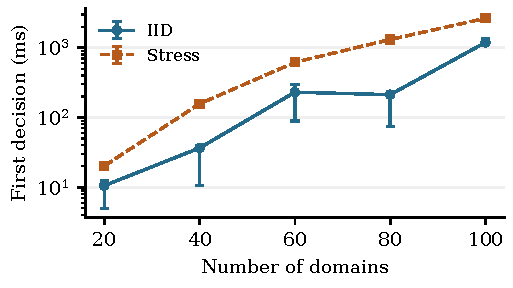
\includegraphics[width=\columnwidth]{results/figures/synthetic_scaling.pdf}
\caption{First online decision time for IID and low-feasibility stress instances. Points are medians of three instances and bars show observed ranges, not confidence intervals.}
\label{fig:scaling}
\end{figure}
We also measure the first decision on 30 larger problems, with $N=20,40,60,80,100$. Above 16 active domains the methods share the same one-step planning mode. The stress family contains many feasible skips and screening candidates, increasing the number of plans to examine. Figure~\ref{fig:scaling} shows median times at 100 domains of 1.19~s (IID) and 2.64~s (stress). Polynomial complexity therefore does not automatically imply suitability for time-critical control. These measurements characterize the Python/Numba implementation on the test hardware. They exclude communication and neither measure later decisions on large problems nor establish their solution quality.

\begin{figure*}[t]
\centering
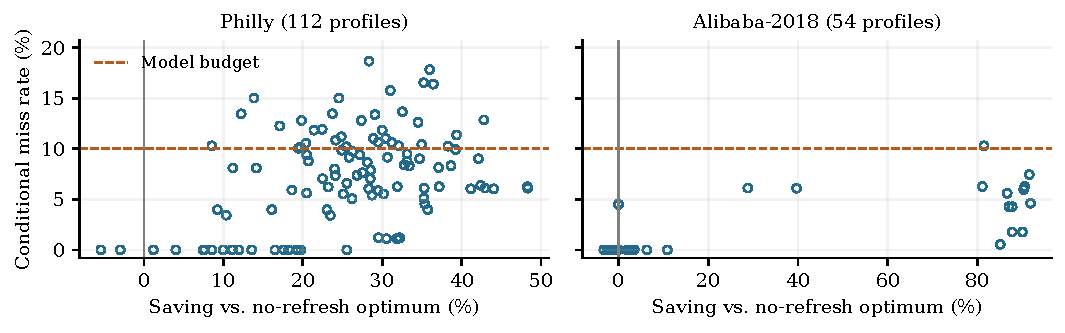
\includegraphics[width=0.94\textwidth]{results/figures/telemetry_cost_risk.pdf}
\caption{Final PSA1-S with model risk tolerance $\varepsilon=0.10$: realized savings and conditional misses across frozen telemetry profiles. Alibaba uses per-lag known samples. Eighteen Alibaba profiles have zero no-refresh cost, so their relative savings are undefined and they are omitted. Profiles share test observations; points are not independent replicates.}
\label{fig:tracerisk}
\end{figure*}
\subsection{Replay with measured resource telemetry}
We next test discovery with measurement-derived information. We use public Microsoft Philly GPU traces~\cite{jeon2019philly,phillyrepo} and Alibaba Cluster Trace v2018~\cite{alibaba2018}. For each dataset we construct three layouts of four domains, each containing two machines selected by training-period coverage. Philly groups are constructed for the experiment, whereas Alibaba groups follow source failure-domain labels. They are not assumed to be administrative federations.

In Philly a machine is feasible if at least two (or four) measured GPU channels have utilization at most 20\% and the free host-memory fraction is at least 5\%. In Alibaba we require an operational \texttt{USING} machine with CPU and normalized memory utilization at or below thresholds A ($40/70$\%), B ($60/80$\%) or C ($80/90$\%). A domain is feasible if either machine meets the predicate. These are availability indicators, not confirmed allocation offers. Host memory does not measure free GPU VRAM.

At test time $t$, a query reveals the recorded predicate $X_i(t)$, while a refresh reveals the older binary signal $Y_i(t)=X_i(t-\Delta)$. Neither is revealed to the policy in advance, and the current state is held fixed during the episode. We fit priors and observation-channel parameters from earlier complete pairs using smoothed frequencies. Philly uses a pre-test fit or weekly re-estimation from the preceding 14 days, whereas Alibaba separates training, calibration and testing chronologically (Appendix~\ref{app:experiments}). Missing values are not treated as negative states. The planner assumes independence across domains, but replay uses the actual joint measurements to evaluate cost and misses.

\begin{table}[t]
\caption{Final PSA1-S replay: savings over optimal no-refresh discovery when $\varepsilon=0$ (\%). One-minute signal, $q=(4,2,1,3)$, $r_i=0.05q_i$. All rows have zero observed misses.}
\label{tab:tracezero}
\centering
\begin{tabular}{lrrr}\hline
 Predicate & Layout 1 & Layout 2 & Layout 3\\\hline
 Philly: two GPUs & 14.38 & 17.27 & 21.15\\
 Philly: four GPUs & 6.85 & 13.89 & 18.73\\
 Alibaba: C (CPU/memory) & 2.54 & 3.52 & 3.04\\\hline
\end{tabular}
\end{table}
\paragraph{Savings without allowing residual risk (RQ1)}
We set $\varepsilon=0$ to test the value of information without accepting any modeled risk of overlooking a resource. Table~\ref{tab:tracezero} uses a one-minute signal and heterogeneous query costs. The Philly layouts provide 61,185, 62,788 and 64,129 primary test points, and Alibaba C provides 24,010, 24,059 and 23,286 per-lag test points. Savings over the same-budget no-refresh optimum range from 14.38 to 21.15\% for two GPUs, from 6.85 to 18.73\% for four GPUs, and from 2.54 to 3.52\% for Alibaba C. No misses occur in these nine comparisons. With positive smoothed beliefs and zero tolerance, imperfect refresh alone cannot rule out a domain. The savings instead come from adapting acquisition and query order to observations, as anticipated by the ordering-probe result.

Since $N=4\le K$, PSA1-S uses exact DP throughout. Its expected model cost matches the exact reference in all 1,220 saved model variants, verified by enumerating 256 truth/signal combinations per model. These replays test the decision model, not the benefit of selective lookahead.

\paragraph{Information quality (RQ4)}
An earlier factorial study of base PSA1 evaluated 180 common base instances under 27 combinations of signal accuracy, refresh cost and risk tolerance. With $\varepsilon=.10$ and $r_i/q_i=.20$ fixed, savings over exact no-refresh discovery increase from 4.0 to 10.7 and 32.2\% as $\alpha_i=\beta_i$ increases from .70 to .85 and .97. The comparison illustrates the importance of signal quality, but is not a benchmark of PSA1-S.

The telemetry grids also contain cases of negative savings. At $\varepsilon=0$ the minimum is $-8.15$\% for Philly and $-3.51$\% in Alibaba's per-lag profiles. For the first Philly layout with two GPUs, rolling fitting and Table~\ref{tab:tracezero}'s costs, increasing the signal age from 1 to 5, 15 and 60 minutes changes savings from 14.38 to 12.46, 11.73 and 8.76\%, respectively, on common test points. This illustrates how older information may be less valuable. It is not a general monotonicity result. A policy optimal for the fitted model need not reduce costs on subsequent measurements.

\subsection{Risk transfer and limitations of calibration}
\label{sec:risktransfer}
Allowing unsuccessful stops at nonzero risk tolerance can produce larger savings, but those savings must be interpreted together with missed resources. Consider the first Philly layout with two GPUs, rolling fitting, a one-minute signal, heterogeneous costs, $r_i/q_i=0.05$ and $\varepsilon=0.10$. The realized mean cost falls from 3.8356 for query-only to 3.7063 for optimal no-refresh discovery and 2.1151 for PSA1-S. The last represents a 42.93\% saving over no-refresh discovery, but 630 of its 10,308 unsuccessful stops miss a feasible domain (6.11\%). No-refresh discovery has zero misses among 9,678 unsuccessful stops. The model tolerances are identical, not the observed risks.

Although every enumerated unsuccessful termination satisfies the model STOP constraint, observed conditional miss rates exceed 10\% in 34 of 112 Philly profiles and one of 54 Alibaba profiles (Fig.~\ref{fig:tracerisk}). The highest observed rates are 18.67\% for Philly (1,996/10,692) and 10.30\% for Alibaba (2,412/23,425). Descriptive 95\% moving-block intervals are [13.41, 25.06]\% and [4.26, 16.75]\%, respectively, using seven-day and one-hour calendar blocks. They account for some temporal dependence but are neither simultaneous bounds across profiles nor guarantees for future data.

One possible source is inaccurate beliefs. For Alibaba's C predicate with a one-minute signal, the aggregate training prior is 0.756 but the test feasibility frequency is 0.497. Refresh improves prediction: the mean test Brier score (squared probability error) drops from 0.327 to 0.100. Yet even a more conservative risk tolerance selected on a separate calibration period (Appendix~\ref{app:experiments}) does not eliminate the worst observed exceedance. Better average probability estimates need not be calibrated at the particular states where the policy stops.

To isolate one possible mechanism, an earlier controlled study of base PSA1 shifted the true log-odds by $\delta$ while leaving the planning model and observation channel fixed. Across 375 base instances, aggregate conditional misses rise from 9.3\% at $\delta=0$ to 14.5, 22.0 and 32.1\% at $\delta=.5,1,1.5$. At zero shift each instance satisfies its own model budget (mean 12.15\%). Underestimating feasibility can therefore undermine the stopping guarantee when the true distribution differs from the planner's beliefs. The telemetry discrepancies could also reflect temporal change, estimation error and cross-domain dependence. The experiments do not identify their separate causal contributions.

\section{Discussion and Conclusion}
\label{sec:discussion}
A central implication for federated discovery is that a summary refresh should be judged by what it changes in the next decision, not by freshness or prediction accuracy alone. A negative signal may make it acceptable to leave a domain unexamined. Even when this is not allowed, an informative signal can change which query is performed first and thus avoid later queries upon an early success. The zero-tolerance telemetry comparisons illustrate this second mechanism with measured resource states and normalized acquisition costs.

The algorithm makes computational effort a design choice. Exact continuation exploits the shrinking search problem, and selective lookahead concentrates work on competing actions. The synthetic results favor this combination over full refinement when decision time matters, but difficult skip-boundary instances retain appreciable gaps. Large-instance timings also suggest limits for time-critical control.

Reliable stopping requires more than an efficient optimizer. The posterior bound guides termination under the assumed model, but inaccurate beliefs can invalidate it as a bound on actual misses. Even improved average prediction is insufficient. Operational assurance requires calibration at the states where the policy actually stops.

We isolate the decision mechanism by considering one intent seeking one suitable resource, fixed feasibility within an episode, conditionally independent domains, at most one binary refresh per domain, definitive queries and known action costs. The telemetry groups are constructed offline, the costs are normalized, and meeting a utilization predicate does not certify admission or reservation. Extensions to correlated or interval-valued beliefs, online calibration under staleness, repeated or continuous observations and competing intents would broaden the model. Measurements of cross-domain communication and allocation outcomes are also needed to evaluate deployment.

In conclusion, discovery involves decisions about both resources and information. Our structural results explain when cheap observations can save expensive queries, and PSA1-S turns these insights into an implementable policy with a model-conditional cost bound. Trustworthy operational use also requires reliable beliefs about resource availability.

% Main text ends here. Start the supplementary material on a separate page.
\clearpage
\appendices
\section{Proofs of Structural and Rollout Results}
\label{app:proofs}
\textit{Proposition 1:} Given a feasible policy with explicit skips, maintain an internal copy of its committed set without executing any SKIP. At each acquisition, reproduce the original policy's choice and update the internal state using the same observation. The two policies share posterior beliefs for all unresolved domains, including the internally skipped ones, so have the same STOP eligibility and cost on every coupled history. Existing commitments are not undone. Conversely, every skip-free policy is available in the augmented model. Thus their optima coincide. The dense DP enumerates states with local statuses $0,+,-,f$, where $f$ is query failure. Each nonterminal transition advances a local status in this order (a refresh goes from $0$ to either sign). Enumerating in reverse order computes the values once. The exact no-refresh DP at state $U$ uses the first term of the Bellman recursion only, with $U\setminus\{i\}$ after failure; a feasible STOP has value zero.

\textit{Proposition 2:} For adjacent modules $i,j$, the difference between the nominal pair costs in the two orders is $c_i+(1-z_i)c_j-c_j-(1-z_j)c_i=c_i z_j-c_j z_i$. All subsequent modules are reached with the same probability $(1-z_i)(1-z_j)$ in either order. Hence swapping an inverted adjacent pair cannot increase cost. For queries, $c_i=q_i,z_i=b_i$.

\textit{Proposition 3:} The three nominal costs are $q_i+(1-p_i)q_j$, $r_i+g_iq_i+(1-p_i\alpha_i)q_j$, and $q_j+(1-p_j)(r_i+g_iq_i)$. Subtracting the first and third, respectively, from the second gives the two strict inequalities in~\eqref{eq:screenband}.

\textit{Proposition 4:} For any fixed query permutation the conditional expected cost averaged over the refresh outcomes equals its pre-refresh expected cost by the law of total expectation. Choosing the optimal order after each outcome cannot cost more than executing the prior optimal order, giving $\Delta_i^{\mathrm{ord}}\ge0$. If no index is crossed, a common optimizing permutation exists (under the stated no-tie assumption); the inequality is then equality. For two domains with $q_i/p_i^+<q_j/p_j<q_i/p_i^-$, the refresh-and-reorder cost is
\begin{equation}
 C_{\mathrm{probe}}=r_i+(1-p_jh_i)q_i+(1-p_i\alpha_i)q_j.
\end{equation}
It strictly beats both fixed query orders iff $r_i$ is less than each of $p_jh_iq_i-p_i(1-\alpha_i)q_j$ and $p_i\alpha_iq_j-p_jg_iq_i$.

\textit{Base supersolution:} Take a nominal plan achieving $H(s)$. Its first action is either the upfront skip, a query, or the refresh beginning its screening module. Following the first action, each nonterminal branch has a feasible remaining plan in the continuation family, or a plan with the same modules in possibly suboptimal order. A positive screening observation leaves a query; a negative observation leaves an admissible skip and the remaining queries. Reordering the remaining modules optimally cannot increase the nominal cost. If STOP has become admissible, $H$ equals zero instead. Thus the cost of the first action plus the expected successor $H$ is at most the initial nominal cost. Minimizing over actions proves $TH\le H$; feasibility and truncation at STOP give $V^*\le H$ and $V^*\le TH$.

\textit{Theorem 1:} Since $m$ never increases, $TB_K=B_K$ in the exact region and $TB_K\le TH\le H=B_K$ elsewhere. Monotonicity of $T$ gives $V^*\le T^2B_K\le TB_K\le B_K$, hence each refined score is no greater than its one-step counterpart. Therefore $M\le TB_K$. At terminal states $V^{\pi_S}=M=0$. Suppose $V^{\pi_S}(s')\le M(s')\le TB_K(s')\le B_K(s')$ at every successor. In the exact region the selective policy executes the exact policy thereafter. Otherwise the chosen action's score uses either $B_K$ or $TB_K$ at the successors, both upper bounds on their policy costs by the induction hypothesis. It follows that $V^{\pi_S}(s)\le M(s)$. Induction on the finite acyclic graph proves~\eqref{eq:guarantee}. No inherited horizon is necessary for this depth-one/two mixed-score bound.

\section{Algorithmic and Implementation Details}
\label{app:algo}
The decision sequence is summarized in Fig.~\ref{fig:psa1s-flowchart}; the pseudocode below specifies the action selection at an individual state.

% Conceptual guide for the Appendix B algorithmic details; the pseudocode remains authoritative.
% IEEE two-column float, TikZ source in results/figures/.
\begin{figure*}[!t]
\centering
% PSA1-S conceptual online-decision flowchart
% Requires: \usepackage{tikz}, \usetikzlibrary{arrows.meta,calc,shapes.geometric}
% Designed to fit an IEEE two-column figure* at its natural size.
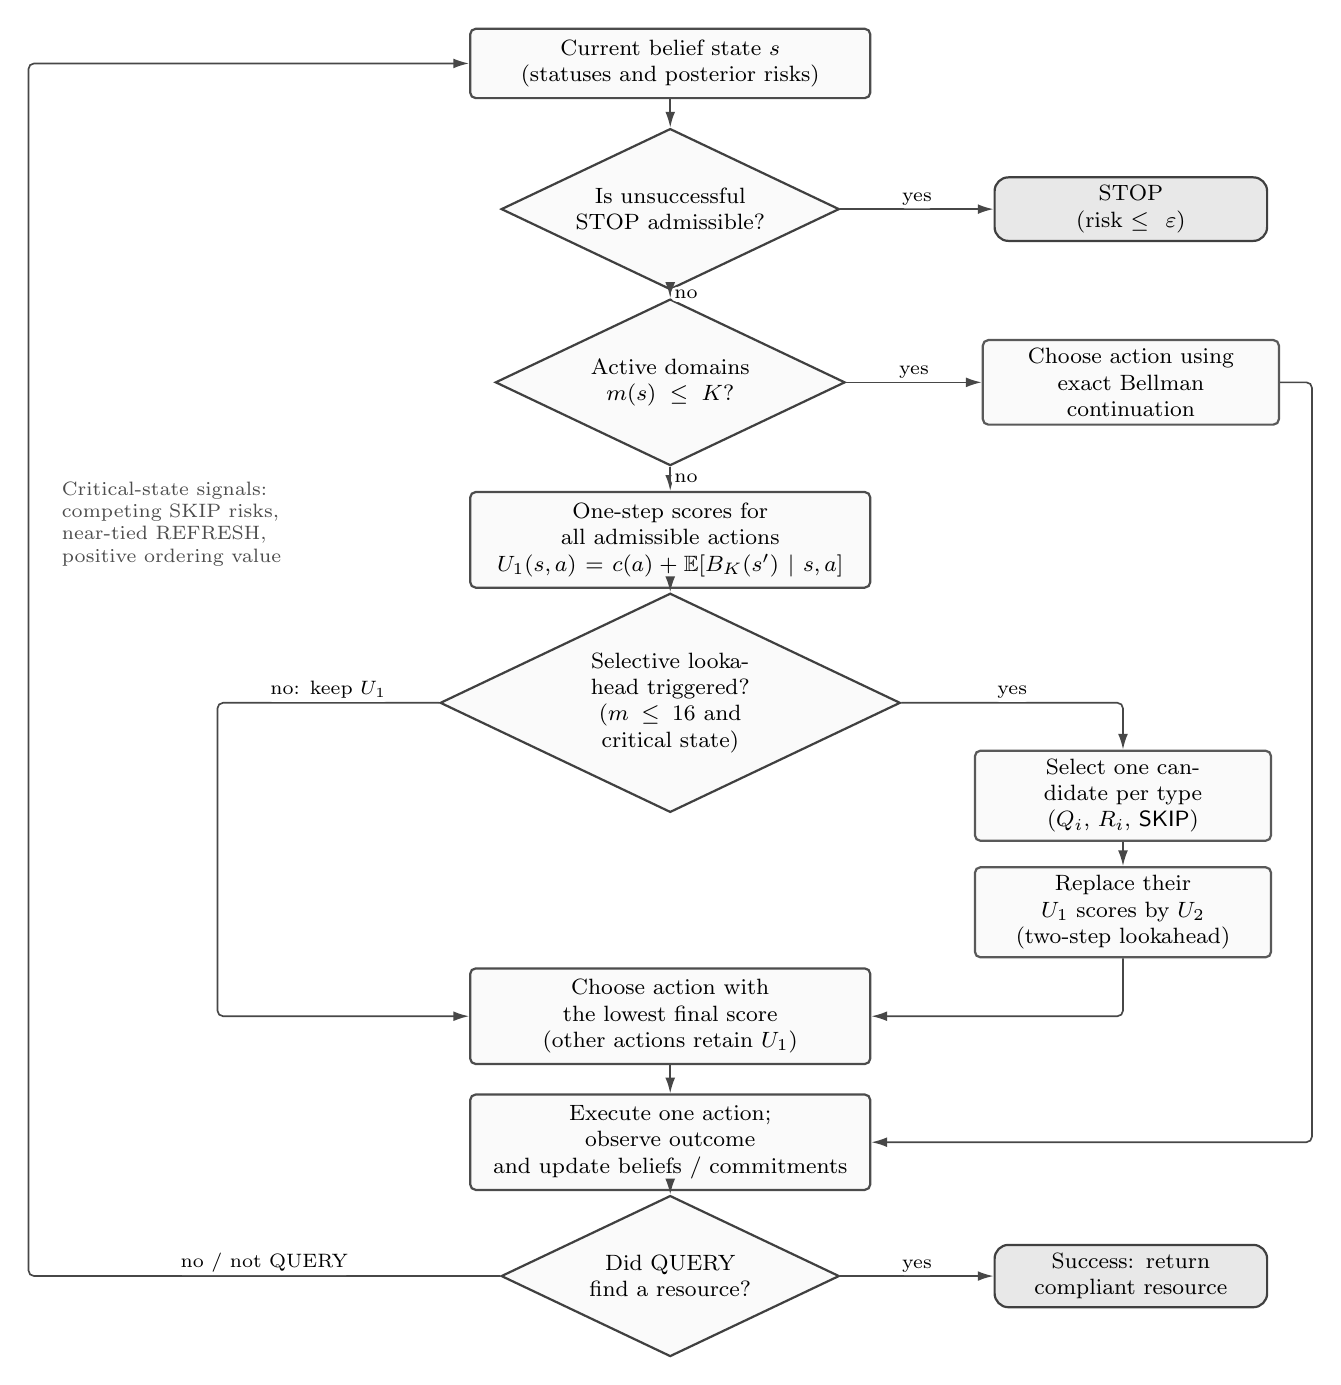
\begin{tikzpicture}[
  font=\footnotesize,
  >={Latex[length=2mm,width=1.25mm]},
  flow/.style={->,semithick,draw=black!72,rounded corners=2pt},
  process/.style={draw=black!70,rounded corners=2pt,thick,fill=black!2,align=center,
                  text width=4.8cm,minimum height=0.69cm,inner sep=4pt},
  smallbox/.style={draw=black!65,rounded corners=2pt,thick,fill=black!2,align=center,
                   text width=3.55cm,minimum height=0.68cm,inner sep=3pt},
  test/.style={draw=black!75,thick,diamond,aspect=2.1,fill=black!2,
               align=center,text width=2.9cm,inner sep=1.3pt},
  finish/.style={draw=black!75,rounded corners=5pt,thick,fill=black!9,
                 text width=3.25cm,minimum height=0.65cm,align=center,inner sep=3pt},
  edgehint/.style={font=\scriptsize,fill=white,inner sep=1.2pt},
]
% Main decision spine: separated so that the decision nodes and arrows remain readable.
\node[process] (state) at (0,0) {Current belief state $s$\\(statuses and posterior risks)};
\node[test] (stop) at (0,-1.85) {Is unsuccessful STOP admissible?};
\node[finish] (done) at (5.85,-1.85) {STOP\\(risk $\leq\varepsilon$)};
\node[test] (tail) at (0,-4.05) {Active domains $m(s)\leq K$?};
\node[smallbox] (exact) at (5.85,-4.05) {Choose action using\\exact Bellman continuation};
\node[process] (scores) at (0,-6.05) {One-step scores for all admissible actions\\$U_1(s,a)=c(a)+\mathbb E[B_K(s')\mid s,a]$};
\node[test] (gate) at (0,-8.12) {Selective lookahead triggered?\\($m\leq16$ and critical state)};
\node[smallbox] (refine) at (5.75,-9.30) {Select one candidate per type\\($Q_i$, $R_i$, \textsf{SKIP})};
\node[smallbox] (newscore) at (5.75,-10.78) {Replace their $U_1$ scores by $U_2$\\(two-step lookahead)};
\node[process] (choose) at (0,-12.10) {Choose action with the lowest final score\\(other actions retain $U_1$)};
\node[process] (execute) at (0,-13.70) {Execute one action; observe outcome\\and update beliefs / commitments};
\node[test] (success) at (0,-15.40) {Did QUERY find a resource?};
\node[finish] (found) at (5.85,-15.40) {Success: return\\compliant resource};
% Spine and branching
\draw[flow] (state)--(stop);
\draw[flow] (stop.east)--node[edgehint,above]{yes}(done.west);
\draw[flow] (stop.south)--node[edgehint,right]{no}(tail.north);
\draw[flow] (tail.east)--node[edgehint,above]{yes}(exact.west);
\draw[flow] (tail.south)--node[edgehint,right]{no}(scores.north);
\draw[flow] (scores)--(gate);
% The negative trigger branch keeps all one-step scores.
\draw[flow] (gate.west)--node[edgehint,above]{no: keep $U_1$}(-5.75,-8.12)
 --(-5.75,-12.10)--(choose.west);
% The positive trigger branch refines at most one candidate of each type.
\draw[flow] (gate.east)-|node[edgehint,above,pos=.25]{yes}(refine.north);
\draw[flow] (refine)--(newscore);
\draw[flow] (newscore.south) |- (choose.east);
\draw[flow] (choose)--(execute);
\draw[flow] (execute)--(success);
\draw[flow] (success.east)--node[edgehint,above]{yes}(found.west);
% The exact-tail branch bypasses heuristic evaluation and selection.
\draw[flow] (exact.east)--(8.15,-4.05)--(8.15,-13.70)--(execute.east);
% Receding-horizon replanning after a failed query, refresh or skip.
\draw[flow] (success.west)--node[edgehint,above]{no / not QUERY}(-8.15,-15.40)
  --(-8.15,0)--(state.west);
% Concise explanation of the three trigger mechanisms.
\node[font=\scriptsize,align=left,anchor=west,text=black!70] at (-7.85,-5.85)
  {Critical-state signals:\\competing SKIP risks,\\near-tied REFRESH,\\positive ordering value};
\end{tikzpicture}

\caption{Online decision flow of PSA1-S. An admissible unsuccessful \STOP{} is selected at zero additional cost. With at most $K$ active domains, the next action is chosen by exact dynamic programming. Otherwise, one-step scores are computed for all admissible actions, and a critical-state trigger can select up to one \QUERY{}, \REFRESH{}, and \SKIP{} candidate for a deeper evaluation. Only one action is executed before replanning. The figure summarizes decision logic; the exact trigger thresholds are specified in the text of Appendix~\ref{app:algo}.}
\label{fig:psa1s-flowchart}
\end{figure*}

For a sorted list of $m$ modules, define prefix cost $P_j=\sum_{k=1}^{j}c_k\prod_{\ell<k}(1-z_\ell)$, survival $L_j=\prod_{k=1}^j(1-z_k)$, and suffix cost $W_j=c_j+(1-z_j)W_{j+1}$, with $P_0=0,L_0=1,W_{m+1}=0$. Removing module $j$ leaves cost $P_{j-1}+L_{j-1}W_{j+1}$. For each of the $m+1$ alternatives (no screen or one screen), sort once, build these arrays, then test feasible singleton upfront skips in constant time each. Exclude the screen itself from deletion and require the combined negative-screen and direct-skip risk to be admissible. This proves the base complexity. The exact table uses an index with two bits per active domain. Tail tables keyed by skipped statuses and active domain sets can be reused across refreshed posteriors and query failures, using failure statuses for removed domains in a cached superset. The implementation uses a 32 MiB LRU budget for these tables only; other memoization is not bounded by this budget.

\noindent\textbf{PSA1-S: one decision at state $s$}
\begin{algorithmic}[1]
\IF{STOP is admissible} \RETURN STOP \ENDIF
\IF{$m(s)\le K$} \RETURN exact DP action \ENDIF
\FOR{each admissible action $a$}
\STATE $u(a)\gets c(a)+\mathbb E[B_K(s')\mid s,a]$
\ENDFOR
\IF{$m(s)\le16$ and a trigger fires}
\FOR{each available type $t\in\{Q,R,\mathrm{SKIP}\}$}
\STATE $a_t\gets\arg\min_{a:\,\mathrm{type}(a)=t}u(a)$
\STATE $u(a_t)\gets c(a_t)+\mathbb E[(TB_K)(s')\mid s,a_t]$
\ENDFOR
\ENDIF
\RETURN $\arg\min_a u(a)$
\end{algorithmic}
The three triggers are an OR condition: (i) at least three active domains and two unused refreshes, positive remaining log-budget $b=B-\sum_{i\in S}w_i$, and two individually admissible strictly positive finite skip weights with $|w_i+w_j-b|\le0.12b$; (ii) the best REFRESH score lies within $0.03\max(\min_a U_1(s,a),10^{-12})$ of the overall best score; (iii) a refresh crosses a query index and has $\Delta_i^{\rm ord}-r_i>10^{-10}$. For PSA1-A all actions are refined when triggered. The implementation rounds rollout scores to 12 decimal places for ranking, breaks ties in the order STOP, SKIP, QUERY, REFRESH and then domain index, and uses an absolute $10^{-12}$ risk tolerance. The exact tail visits domains in index order, trying query before refresh and updating on strict improvement. The mathematical statements use exact arithmetic and exact minimization. The parameters and numerical rules are those of the frozen benchmark.

\section{Belief Construction Interface}
\label{app:belief}
The decision model does not require a specific estimator. For instance, an intent induces a feasible region $\mathcal F(I)$ in resource-attribute space. For domain $i$, resource class $c$ with $n_{ic}$ members and conditional per-resource feasibility probability $\theta_{ic}(I)=\Pr(\mathbf Z_{ic}\in\mathcal F(I)\mid\mathcal K_i,I)$, conditional independence of members gives
\begin{equation}
 p_i(I)=1-\prod_c(1-\theta_{ic}(I))^{n_{ic}}.
\end{equation}
This product is illustrative, not valid in general for correlated members. A latent common domain state can instead yield a mixture of conditional products. A refresh updates the summary and its induced belief; the binary channel in~\eqref{eq:bayes} abstracts this update. In the telemetry replay, rather than imposing a class independence model, $X_i(t)$ is a measured group-level feasibility predicate and $Y_i(t)=X_i(t-\Delta)$ is a delayed signal revealed only by REFRESH. Empirical training frequencies estimate $p_i,\alpha_i,\beta_i$ from available past pairs. This preserves within-group dependencies in the predicate but does not validate the across-domain independence assumption. Estimator details and chronological splits belong in the experimental appendix; calibration drift is a separate issue from model-based risk feasibility.

\section{Experimental Methodology and Reproducibility}
\label{app:experiments}
\subsection{Synthetic benchmark design}
The controlled benchmark isolates algorithmic behavior under a known independent-domain model. It contains ten independently seeded instances for each of three families at $N\in\{8,10,12\}$ (90 instances). The \emph{IID} family samples broadly varying beliefs, costs and observation quality. The \emph{boundary} family places the risk threshold near the joint feasibility probability of two low-probability domains, making competing skips consequential. The \emph{probe} family combines informative, low-cost refreshes with a strict stopping budget to exercise adaptive ordering; it does not force an ordering reversal.

Let $\mathcal U[a,b]$ denote a uniform draw. IID samples $p_i\sim\mathcal U[.05,.85]$, $\log_{10}q_i\sim\mathcal U[-.2,1.1]$, $\log_{10}(r_i/q_i)\sim\mathcal U[-1.4,.15]$, $\alpha_i,\beta_i\sim\mathcal U[.65,.995]$, and $\varepsilon\in\{.01,.03,.05,.1,.2,.3\}$ uniformly. Boundary instances draw $t\sim\mathcal U[.06,.19]$, $p_1\sim\mathcal U[.015,.035]$, and set $p_2=(t-p_1)/(1-p_1)$, so the first two domains have joint feasibility probability $t$. They draw $p_3\in[.25,.65]$, $p_4\in[.22,.6]$, $q_{1:4}$ from $[13,25]$, $[12,24]$, $[2,6]$, $[3,8]$, respectively, $r_i/q_i\in[.045,.17]$, $\alpha_i\in[.8,.97]$, $\beta_i\in[.82,.96]$, and set $\varepsilon=t\pm\min(.003,.015t)$. Remaining domains use $p_i\in[.04,.32]$, $q_i\in[2,12]$ and $r_i/q_i\in[.05,.30]$, with the same channel ranges. Probe draws $p_i\in[.18,.7]$, $q_i\in[2,14]$, $r_i/q_i\in[.015,.15]$, $\alpha_i\in[.78,.95]$, $\beta_i\in[.8,.97]$, and fixes $\varepsilon=.005$. All unqualified intervals in this paragraph denote independent uniform draws; seed parity selects the boundary side.

All methods use the same generated instances. Expected policy costs are evaluated over complete model policy trees against exact DP, while online times use two shared, independently sampled worlds per instance. Separate $N=20$--100 timing tests include a low-feasibility stress family ($p_i\in[.018,.026]$, $q_i\in[4,12]$, $r_i=.2q_i$, $\alpha_i=\beta_i=.95$, $\varepsilon=.1$). Benchmark seeds are $73100000+10000N+1000f+j$ (family index $f=0,1,2$; $j=0,\ldots,9$). Timing-world seeds are $100\,\mathrm{seed}+k$ ($k=0,1$). Timing used AMD EPYC 9V74, Python 3.13.5, NumPy 2.3.5 and Numba 0.65.1, after JIT warm-up.

\subsection{Telemetry preprocessing and belief estimation}
We construct three four-domain layouts per dataset, each domain containing two machines chosen using training-period coverage, never test-policy performance. The public Philly GPU and Alibaba-2018 CPU--memory traces yield offline binary feasibility predicates, not verified allocation offers. A query reveals the current recorded predicate $X_i(t)$; a refresh reveals $Y_i(t)=X_i(t-\Delta)$ only after that action. Each episode freezes $X_i(t)$. Unknown measurements are not treated as failures, and no utilization interpolation is performed.

Philly uses completed one-minute bins and 24 machines assigned to three disjoint eight-machine layouts. Static fitting uses observations before 2017-11-01 07:00 UTC; testing starts at 08:00 UTC. The rolling alternative refits weekly on the preceding 14 days, falling back to the static estimate with fewer than 100 known pairs. Signal ages are $\Delta\in\{1,5,15,60\}$ minutes. Alibaba uses ten-second bins and source failure-domain labels to form 12 two-machine groups. Its disjoint chronological intervals are training $[0,3)$ days, calibration $[3\,\mathrm d+1\,\mathrm h,5\,\mathrm d)$, and testing $[5\,\mathrm d+1\,\mathrm h,8\,\mathrm d)$, with $\Delta\in\{1,10,60\}$ minutes; per-lag known masks and common masks are analyzed separately.

From $n$ known current/delayed pairs, let $n_1,n_0$ count positive/negative current states, and $n_{11},n_{00}$ the correctly positive/negative delayed observations. Laplace-smoothed estimates are $p=(n_1+1)/(n+2)$, $\alpha=(n_{11}+1)/(n_1+2)$ and $\beta=(n_{00}+1)/(n_0+2)$. Both datasets use normalized query costs $q=(1,1,1,1)$ or $(4,2,1,3)$, with $r_i=.05q_i$; Philly also includes a $.20q_i$ subgrid. These are experimental costs, not measured network signalling times. The resulting four-domain problems use the exact tail of PSA1-S ($K=8$), not selective lookahead.

\subsection{Evaluation, uncertainty, and calibration}
Synthetic comparisons report expected-cost gaps to exact DP and savings over exact, same-budget no-refresh discovery. The final benchmark uses a paired bootstrap stratified by family and size (10,000 resamples). On telemetry, we replay each policy against recorded joint outcomes and measure realized mean action cost and conditional misses $M/E$, where $E$ is the number of unsuccessful terminations and $M$ is the number that overlooked a recorded feasible domain. This rate is distinct from both the model-posterior STOP bound and the unconditional miss rate. Undefined ratios (zero denominators) are not assigned values.

For Alibaba, a separate calibration interval selects the largest budget in $\{.01,.025,.05,.075,.1\}$ that yields at least 200 unsuccessful calibration stops and at most 5\% empirical conditional misses, or zero if none qualifies. This choice is frozen before testing and does not certify future risk. Descriptive 95\% moving-block intervals use 1,000 resamples, with seven-day calendar blocks for Philly and one-hour blocks for Alibaba. Across-domain independence remains a planning assumption, not a property imposed on telemetry. Earlier factorial and prior-shift mechanism checks concern the base PSA1, not the final PSA1-S benchmark.

\subsection{Reproducibility scope and planned artifact}
The preserved benchmark results separate model parameters and policy costs (\texttt{holdout.jsonl}), episode timings (\texttt{online.jsonl}), and large-instance root timings (\texttt{scaling.jsonl}). The telemetry evaluation preserves the original processing/replay scripts, fitted beliefs, observation masks and provenance, together with the zero-budget controls (\texttt{paper\_primary\_zero\_budget.csv}) and final-policy results (\texttt{paper\_final\_code\_policy\_results.csv}). The reported tables derive from these frozen evaluations rather than newly fitted traces. A versioned GitHub repository and Zenodo archive are planned to provide the code, pinned environment, configuration/seed manifest, public-dataset acquisition instructions, and table/figure reproduction commands. A persistent identifier will be added when that artifact is released.

\begin{thebibliography}{00}
\bibitem{leivadeas2023survey} A. Leivadeas and M. Falkner, ``A survey on intent-based networking,'' \emph{IEEE Commun. Surveys Tuts.}, vol. 25, no. 1, pp. 625--655, 2023, doi: 10.1109/COMST.2022.3215919.
\bibitem{mehmood2025lifecycle} K. Mehmood, K. Kralevska, and D. Palma, ``Knowledge-driven intent life-cycle management for cellular networks,'' \emph{IEEE Trans. Netw. Service Manag.}, vol. 22, no. 5, pp. 4806--4826, 2025, doi: 10.1109/TNSM.2025.3579547.
\bibitem{etsi2024zsm} ETSI, ``Zero-touch network and Service Management (ZSM); Intent-driven autonomous networks; Generic aspects,'' ETSI GR ZSM 011 V2.1.1, Sep. 2024.
\bibitem{murturi2022metadata} I. Murturi and S. Dustdar, ``A decentralized approach for resource discovery using metadata replication in edge networks,'' \emph{IEEE Trans. Services Comput.}, vol. 15, no. 5, pp. 2526--2537, 2022, doi: 10.1109/TSC.2021.3082305.
\bibitem{etsi2025ngsild} ETSI, ``Context Information Management (CIM); NGSI-LD API,'' ETSI GS CIM 009 V1.9.1, Jul. 2025.
\bibitem{montoya2015fedra} G. Montoya, H. Skaf-Molli, P. Molli, and M.-E. Vidal, ``Federated SPARQL queries processing with replicated fragments,'' in \emph{Proc. Int. Semantic Web Conf. (ISWC)}, LNCS 9366, pp. 36--51, 2015.
\bibitem{chiariotti2022qaoi} F. Chiariotti, J. Holm, A. E. Kal\o r, B. Soret, S. K. Jensen, T. B. Pedersen, and P. Popovski, ``Query age of information: Freshness in pull-based communication,'' \emph{IEEE Trans. Commun.}, vol. 70, no. 3, pp. 1606--1622, 2022, doi: 10.1109/TCOMM.2022.3141786.
\bibitem{weitzman1979} M. L. Weitzman, ``Optimal search for the best alternative,'' \emph{Econometrica}, vol. 47, no. 3, pp. 641--654, 1979, doi: 10.2307/1910413.
\bibitem{gkenosis2022sbfe} D. Gkenosis, N. Grammel, L. Hellerstein, and D. Kletenik, ``The stochastic Boolean function evaluation problem for symmetric Boolean functions,'' \emph{Discrete Appl. Math.}, vol. 309, pp. 269--277, 2022.
\bibitem{wei2017imperfect} W. Wei, H. Li, and R. Leus, ``Test sequencing for sequential system diagnosis with precedence constraints and imperfect tests,'' \emph{Decision Support Systems}, vol. 103, pp. 104--116, 2017, doi: 10.1016/j.dss.2017.09.009.
\bibitem{ahmad2014active} S. Ahmad, H. Huang, and A. J. Yu, ``Cost-sensitive Bayesian control policy in human active sensing,'' \emph{Front. Hum. Neurosci.}, vol. 8, Art. 955, 2014, doi: 10.3389/fnhum.2014.00955.
\bibitem{bertsekas1999rollout} D. P. Bertsekas and D. A. Casta\~n\'on, ``Rollout algorithms for stochastic scheduling problems,'' \emph{J. Heuristics}, vol. 5, no. 1, pp. 89--108, 1999, doi: 10.1023/A:1009634810396.
\bibitem{jeon2019philly} M. Jeon, S. Venkataraman, A. Phanishayee, J. Qian, W. Xiao, and F. Yang, ``Analysis of large-scale multi-tenant GPU clusters for DNN training workloads,'' in \emph{Proc. USENIX ATC}, 2019, pp. 947--960.
\bibitem{phillyrepo} Microsoft Research, ``Philly traces,'' public dataset and documentation, 2019. GitHub: \texttt{msr-fiddle/philly-traces}, commit \texttt{29a1b87}, CC BY 4.0.
\bibitem{alibaba2018} Alibaba Cluster Trace Program, ``Alibaba Cluster Trace v2018,'' public dataset, 2018. GitHub: \texttt{alibaba/clusterdata}, \texttt{cluster-trace-v2018}, commit \texttt{3858992}.
\end{thebibliography}


\end{document}
